% Chapter 1

\chapter{Introduction} % Main chapter title

\label{Chapter1} % For referencing the chapter elsewhere, use \ref{Chapter1} 

%----------------------------------------------------------------------------------------

% Define some commands to keep the formatting separated from the content 
\newcommand{\keyword}[1]{\textbf{#1}}
\newcommand{\tabhead}[1]{\textbf{#1}}
\newcommand{\code}[1]{\texttt{#1}}
\newcommand{\file}[1]{\texttt{\bfseries#1}}
\newcommand{\option}[1]{\texttt{\itshape#1}}

%----------------------------------------------------------------------------------------


\section{Recognition tasks}

The study of human intelligence, and the study of artificial
intelligence, form two major intertwining areas of modern research.
The attempt to algorithmically mimic or exceed human perceptual and
cognitive capabilities not only advances the application of artificial
intelligence for industrial applications, but also sheds light on the
nature of biological intelligence, and the nature of intelligence in
general.  One of the key capabilities of an intelligent system,
natural or artificial, is the ability to recognize objects, agents,
and signs in the environment based on input data.  Human brains have a
remarkable ability to recognize objects, faces, spoken syllables and
words, and written symbols or words, and this recognition ability is
essential for everyday life.  While researchers in artificial
intelligence have attempted to meet human benchmarks for these
classical recognition tasks for the last X decades, only very recent
advances in machine learning, such as deep neural networks, have
allowed algorithmic recognition algorithms to approach or exceed human
performance [CITE].

Within the statistics and machine learning literature, the usual
formalism for studying a recognition task is to pose it as a
\emph{multi-class classification} problem.  One delineates a finite
set of distinct entities which are to be recognized and distinguished,
which is the \emph{label set} $\mathcal{Y}$.  The input data is
assumed to take the form of a finite-dimensional real \emph{feature
  vector} $X \in \mathbb{R}^p$.  Each input instance is associated
with exactly one true label $Y \in \mathcal{Y}$.  The solution to the
classification problem takes the form of an algorithmically
implemented \emph{classification rule} $h$ that maps vectors $X$ to
predicted labels $\hat{Y} \in \mathcal{Y}$.  The classification rule
can be constructed in a data-dependent way: that is, one collects a
number of labelled \emph{training observations} $(X_1, Y_1)$ which is
used to inform the construction of the classification rule $h$.  The
success of the classification rule $h$ is measured by the \emph{expected loss} or \emph{risk},
which in the case of zero-one loss takes the form
\[
\text{Risk}(h) = \Pr[h(X) \neq Y],
\]
where the probability is defined with reference to the unknown
population joint distribution of $(X, Y)$.  
%A common approach for
%constructing a classifier $h$ is \emph{empirical risk minimization} [CITE],
%which constructs $h$ by minimizing the objective function
%\[
%\text{EmpiricalRisk}_{h \in \mathcal{H}}(h) = \frac{1}{n} \sum_{i=1}^n I(h(X) \neq Y)
%\]
%where $\mathcal{H}$ is some pre-specified function class.

However, a limitation of the usual multi-class classification
framework for studying recognition problems is the assumption that the
label set $\mathcal{Y}$ is finite and known in advance.  When
considering human recognition capabilities, it is clear that this is
not the case.  Our ability to recognize faces is not limited to some
pre-defined, fixed set of faces; same with our ability to recognize
objects in the environment.  Humans learn to recognize novel faces and
objects on a daily basis.  And, if artificial intelligence is to fully
match the human capability for recognition, it must also possess the
ability to add new categories of entities to its label set over time;
however, at present, there currently exists a void in the machine
learning literature on the subject of the online learning of new
classes in the data [CITE].

The central theme of this thesis is the study of \emph{randomized
  classification}, which can be motivated as an extension of the
classical multi-class classification framework to accommodate the
possibility of growing or infinite label sets $\mathcal{Y}$. The basic
approach taken is to assume an infinite or even continuous label space
$\mathcal{Y}$, and then to study the problem of classification on
finite label sets $S$ which are randomly sampled from $\mathcal{Y}.$
This, therefore defines a \emph{randomized classification} problem
where the label set is finite but may vary from instance to instance.
One can then proceed to answer questions about the variability of the
performance due to randomness in the labels, or how performance
changes depending on the size of the random label set.

An additional set of applications of the randomized classification
framework lies in its connection to information theory.  Randomized
classification is the natural analogue of the \emph{random code}
models first studied by Claude Shannon.  Furthermore, it becomes
possible to prove extensions of Fano's inequality to the case of
continuous $X$ and $Y$ by means of randomized classification.
Therefore, randomized classification can be used as a means of
inferring mutual information.

The rest of the thesis is organized as follows.  The remaining
sections in this chapter deal with background material on supervised
learning and information theory, as well as the application of both to
neuroscience, which forms a major motivation for the current work.
Chapter 2 introduces the concept of randomized classification, and
also establishes some variability bounds which will be used later in
the development of inference procedures.  Chapter 3 studies the
dependence of classification accuracy on the label set size in
randomized classification, and a practical method for predicting the
accuracy-versus-label set size curve from real data.  Chapter 4 and 5
deal with the applications of randomized classification to the
estimation of mutual information in continuous data: chapter 4 derives
a lower confidence bound for mutual information under very weak
assumptions, while chapter 5 works within an asymptotic
high-dimensional framework which leads to a more powerful but less
robust estimator estimate of mutual information.

\section{Information and Discrimination}

In studying the problem of recognition, we make use of two closely
related frameworks: firstly, the multi-class classification framework
from the statistics and machine learning literature, and secondly, the
concepts of information theory.  From a broader perspective, this is
hardly unusual, since concepts such as entropy, divergence, and mutual
information are commonly applied in theoretical statistics and machine
learning.  Furthermore, information theory, theoretical statistics,
and machine learning are based on the same foundation:
measure-theoretic probability theory; one could even say that all
three disciplines are subfields of applied probability.  However,
while the three sub-fields may appear very similar from a mathematical
perspective, some differences arise if we examine the kinds of
intuitions and assumptions that are characteristic of the literature
in each area.

A common problem to all three subfields is the inference of some
unobserved quantity on the basis of observed quantities.  In classical
statistics, the problem is to infer an unknown parameter; in
supervised learning, the problem is to predict an unobserved label or
response $Y$; in information theory, the problem is to decode a noisy
message.  Next, the metric for quantifying achievable performance
differs between the three disciplines.  In classical statistics, one
is concerned with the variance of the estimated parameter, or
equivalently, the Fisher information.  In machine learning, one seeks
to minimize (in expectation) a \emph{loss} function which measures the
discrepancy between the prediction and the truth.  In information
theory, one can measure the quality of the noisy channel (and
therefore, the resulting achievable accuracy) through the \emph{mutual
  information} $I(X; Y)$ between the sender's encoded message $X$ and
the reciever's recieved message $Y$.  If we specialize within machine
learning to the study of classification, then we are concerned with
accurate \emph{discrimination} of the input $X$ according to labels
$Y$.  Similarly, if we specialize to the problem of hypothesis testing
within statistics, the the problem is again to \emph{discriminate}
between two (or more) different hypotheses regarding the
data-geenrating mechanism.

%% have to reorder the next para, 
The concepts of \emph{information} and \emph{discrimination} are quite
distinct from an intuitive standpoint; however, they are linked at a
fundamental level.  This link can be seen throughout statistics and
machine learning, and in the way we think about statistical problems.
A statistical hypothesis test is \emph{informative} because it
provides evidence that the data behaves according to a certain
hypothesis rather than another.  %% slightly redundant with prev para.
In information theory, even if the reciever cannot conclusively
determine the sender's message from the observed signal, the signal
still contains \emph{information} if it contains some evidence that
favors one set of possible messages over another.  The formalism of
measure-theoretic probability theory provides yet another example of
the conceptual link between information and
discrimination\footnote{Supposing $\Omega$ is a probability space
  defined with respect to a $\sigma$-algebra $\mathcal{F}$, we can
  represent our state of knowledge with a filtration (or
  sub-$\sigma$-algebra) $\mathcal{F}' \subseteq \mathcal{F}$.
  Complete knowledge (zero uncertainty) is represented by the full
  $\sigma$-algebra: that is, $\mathcal{F}' = \mathcal{F}$.  Partial
  knowledge is represented by a coarser filtration, $\mathcal{F}
  \subset \mathcal{F}'$.  The filtration, of course, indicates that
  our knowledge is sufficient to \emph{discriminate} the outcome space
  $\Omega$ into a number of finitely or infinitely many categories.
  The more information we have, (or, the closer we come to complete
  knowledge of the outcome), the more finely we can discriminate the
  realized outcomes given by $\omega \in \Omega$.}.

%% the purpose of this paragraph is to make the link between discrimination and information
%% this para needs work after being moved
Either natural or artificially intelligence recognition systems must
rely on input data that is \emph{informative} of the optimal response
if they are to achieve reasonable discriminative accuracy.  In natural
environments, mammals rely on a combination of visual, auditory, and
tactile cues to recognize potential threats in the environment.
Mammalian brains integrate all of this sensory information in order to
make more rapid and reliable decisions.  Generally, increased
diversity and quality of the available sources of information will
lead to more accurate recognition (say, of possible environmental
threats.)

This link between the information content of the input and the
achievable discrimination accuracy was first quantified by Claude
Shannon via the concept of \emph{mutual information.}  The mutual
information $I(X; Y)$ quantifies the information content that an input
$X$ holds abut a target of interest, $Y$.  For instance, in the case
of facial identification, the discrimination target $Y$ is a label
corresponding to the identity of the person, and $X$ is an image of
the individual's face.  An image corrupted by noise holds less
information, and correspondingly leads to lower classification
accuracies.

The discrmination problem that Shannon studied--the
\emph{noisy-channel decoding problem}, is extremely similar to the
multi-class classification problem, but also features some important
differences.  A side-by side comparison between the schematics of
multi-class classification and the noisy channel problem is displayed
in Figure \ref{fig:mcc_vs_it}.  We will elaborate much further on the
comparison illustrated in the figure, but for now, one can note that
both the multi-class classification problem and the noisy-channel
decoding problem involves the inference of a latent variable $Y$ from
an observation $X$, where $X$ is linked to $Y$ through a conditional
distribution $F_Y$.

\tikzstyle{block} = [rectangle, draw, fill=white, 
    text width=5em, text centered, rounded corners, minimum height=4em]
\tikzstyle{cloud} = [ellipse, draw, fill=white, 
    text width=5em, text centered, rounded corners, minimum height=4em]
\tikzstyle{line} = [draw, -latex']
    
\begin{figure}
\centering
\begin{tabular}{ccc}

Multi-class classification & & Information Theory\\

\begin{tikzpicture}[node distance = 2cm, auto]
    % Place nodes
    \node [block] (init1) {label $Y$};
    \node [cloud, below of=init1] (init2) {distribution $F_Y$};
    \node [block, below of=init2] (init3) {observation $X$};
    \node [cloud, below of=init3] (init4) {classification rule $h(X)$};
    \node [block, below of=init4] (init5) {estimate $\hat{Y}$};
    % Draw edges
    \path [line] (init1) -- (init2);
    \path [line] (init2) -- (init3);
    \path [line] (init3) -- (init4);
    \path [line] (init4) -- (init5);
\end{tikzpicture} 

& & 

\begin{tikzpicture}[node distance = 2cm, auto]
    % Place nodes
    \node [block] (initA) {message $M$};
    \node [cloud, below of=initA] (initB) {encoder $g(M)$};
    \node [block, below of=initB] (init1) {encoded message $Y$};
    \node [cloud, below of=init1] (init2) {noisy channel $F_Y$};
    \node [block, below of=init2] (init3) {observation $X$};
    \node [cloud, below of=init3] (init4) {decoder $d(X)$};
    \node [block, below of=init4] (init5) {estimate $\hat{M}$};
    % Draw edges
    \path [line] (initA) -- (initB);
    \path [line] (initB) -- (init1);
    \path [line] (init1) -- (init2);
    \path [line] (init2) -- (init3);
    \path [line] (init3) -- (init4);
    \path [line] (init4) -- (init5);
\end{tikzpicture} 

\end{tabular}
\caption{Comparing the discrimination tasks in multi-class classification and information theory.}
\label{fig:mcc_vs_it}
\end{figure}

We will now briefly review the relevant background for supervised learning and
information theory, to give the context for each side of figure
\ref{fig:mcc_vs_it}.  Afterwards, we will compare and contrast the
supervised learning and information theory, and note what kind of
cross-talk exists between the two related fields, and what new
developments could still arise by way of a dialogue between supervised
learning and information theory.  One such new development is the
\emph{randomized classification} model, since it is a very close
analogue of the \emph{random code} model studied in information
theory.

\subsection{Supervised learning}

Up until now we have been discussing \emph{classification}, which is a
particular type of \emph{prediction task}.  However, the most general
recipe for a prediction task involves:

\begin{itemize}
\item A predictor space $\mathcal{X}$ defining the possible values the predictor $X$ can take;
\item A response space $\mathcal{Y}$ defining the possible values the response $Y$ can take;
\item An \emph{unknown} population joint distribution $G$ for the pair $(X, Y)$;
\item A \emph{loss} function defining the penalty for incorrect
  predictions, $L: \mathcal{Y} \times \mathcal{Y} \to \mathbb{R}$.  If
  $Y$ is the response, and $\hat{Y} = h(X)$ is the prediction, then
  the loss for making the prediction $\hat{Y}$ when the truth is $Y$
  is given by $L(Y; \hat{Y})$.
\end{itemize}

The various types of prediction tasks include classification,
regression, and multivariate variants: such as multi-label
classification and multiple-response regression.  These special cases
are just specializations of the general prediction task to a
particular type of response space.

\begin{itemize}
\item In \emph{classification}, the response space is finite and
  discrete.  In \emph{binary classification}, the response space
  $\mathcal{Y}$ consists of two elements, say, $\mathcal{Y} = \{0,
  1\}$.  Multi-class classification usually refers to the case
  $\mathcal{Y}$ has more than two elements.  The most common loss
  function for classification is zero-one loss,
\[
L(y; \hat{y}) = I(y \neq \hat{y}).
\]
\item In \emph{regression}, the response space is $\mathbb{R}$.  The most common loss function is squared loss:
\[
L(y; \hat{y}) = (y - \hat{y})^2.
\]
\item In \emph{multi-label classification}, the response space is a
  product of several finite sets, say $\mathcal{Y} = \mathcal{Y}_1
  \times \mathcal{Y}_2 \times \cdots \mathcal{Y}_\ell$.  That is to
  say, that the response $\vec{Y}$ consists of a categorical vector,
  $\vec{Y} = (Y_1,\hdots, Y_\ell)$. More complex types of loss
  functions can be considered, such as \emph{Jaccard distance},
\[
L(\vec{y}; \hat{\vec{y}}) = \frac{\sum_{i=1}^\ell y_i \wedge \hat{y}_i}{\sum_{i=1}^\ell y_i \vee \hat{y}_i}.
\]
\item In \emph{multiple-response regression}, the response space is $\mathbb{R}^p$.  A natural loss function is squared Euclidean distance,
\[
L(\vec{y}; \hat{\vec{y}}) = ||\vec{y} - \hat{\vec{y}}||^2.
\]
\end{itemize}

A \emph{prediction rule} is a function $h: \mathcal{X} \to
\mathcal{Y}$ for predicting $Y$ as a function of $X$.  The \emph{risk}
of the prediction rule is the expected loss under the joint
distribution $G$,
\[
\text{Risk}(h) = \mathbb{E}[L(Y; h(X))]
\]

Prediction rules can be found through a variety of means.  In some
domains, experts manually construct the prediction rules using their
domain knowledge.  However, the field of \emph{supervised learning}
aims to algorithmically construct, or `learn' a good prediction rule
from data.  In supervised learning, we assume that we have access to a
\emph{training set} consisting of $n_1$ observations
$\{(X_i,Y_i)\}_{i=1}^{n_1}$, plus a \emph{test set} consisting of
$n_2$ observations $\{(X_i,Y_i\}_{i=n_1 + 1}^{n_1 + n_2}$; usually, we
assume that the pairs in both the training and test set have been
sampled i.i.d. from the distribution $G$.  We will also write $\bX$
for the matrix of training observations, with each $X_i$ stacked in
rows, and $\bY$ for the vector of training responses. The training set
is used to construct the prediction rule $h$.  The test set is then
used to estimate the risk of the constructed rule (which is also
called the \emph{generalization error}.)

A \emph{learning algorithm} $\Lambda$ is a procedure for constructing the
prediction rule $h$ given training data $\{(X_i,Y_i)\}_{i=1}^{n_1}$ as
an input.  Formally, we write
\[
h = \Lambda(\{(X_i,Y_i)\}_{i=1}^{n_1}),
\]
indicating that $h$ is the output of the function $\Lambda$ evaluated
on the input $\{(X_i,Y_i)\}_{i=1}^{n_1}$.  How learning algorithms are
implemented in practice can very considerably; we illustrate just a
few of the most common types of learning algorithms:

\begin{itemize}
\item \emph{Parametric generative models.}  Define a parametric family
  $F_\theta$ of joint distributions $(X, Y)$.  For instance, in linear
  regression, a commonly studied family is the multivariate normal linear model,
  where
\[
(X, Y) \sim N((1,0,\hdots,0, \beta_0), \begin{pmatrix}\Sigma_X & \Sigma_X \beta \\
\beta^T \Sigma_X & \beta^T \Sigma_X \beta + \Sigma_\epsilon\end{pmatrix},
\]
or equivalently,
\[
X \sim N((1,0,\hdots,0), \Sigma_X)
\]
\[
Y|X \sim N(X \beta, \Sigma_\epsilon).
\]
The learning algorithm $\Lambda$ proceeds by first fitting the
parametric model to estimate the parameter $\hat{\theta}$.  A variety
of methods may be chosen to estimate $\theta$: maximimum likelihood,
penalized maximum likelihood, or Bayesian estimation.  Note also that
in many cases, such as regression, not all parameters of the model
need to be estimated for prediction purposes.  For instance, in the
linear regression model given above, only $\beta$ needs to be
estimated, and not $\Sigma_X$ or $\Sigma_Y$.  One then constructs the
prediction rule $h$ depending on the estimated parameter
$\hat{\theta}$, in a way so that the risk is controlled.  For
instance, in linear regression, one takes $h = \hat{\beta}^T X.$
\item \emph{Empirical risk minimization.} As mentioned before, define
  a function class $\mathcal{H}$.  We wish to search for an element $h
  \in \mathcal{H}$ which minimizes the empirical risk on the training
  set,
\[
h = \text{argmin}_{h \in \mathcal{H}} \frac{1}{n_1} \sum_{i=1}^{n_1} \tilde{L}(Y_i, h(X_i))
\]
Here, $\tilde{L}$ could be taken to be equal to the original loss
function $L$, or could be taken to be a different function, such as a
smoothed approximation of $L$.  The advantage of using a smoothed
approximation $\tilde{L}$ is that the empirical risk can be made
differentiable (whereas the original loss $L$ might be
nondifferentiable) and hence the optimization made much more tractable
from a numerical standpoint.  This is often the case in binary
classification, where $L$ is zero-one loss, but $\tilde{L}$ is the logistic loss
\[
\tilde{L}(y; p) = y \log p + (1-y) \log (1-p).
\]
%% might have to explain why the prediction space is probabilities rather than responses, as well
\end{itemize}
Further complicating the picture is the fact that often the learning
algorithm requires specification of various \emph{hyperparameters}.
For instance, lasso regression is a penalized generative model which
finds $\beta$ minimizing the objective function
\[
\beta = \text{argmin}_\beta \frac{1}{2}||\bY - \bX \beta||^2 + \lambda ||\beta||_1.
\]
and then constructs the prediction rule
\[
h(x) = x^T \beta.
\]
%% No explanation of L1 norm notation
Here, the L1-penalty constant $\lambda$ needs to be specified by the
user.  In practice, one can either use prior knowledge or
theoretically-justified rules to select $\lambda$; or, more commonly,
one uses various procedures to automatically tune $\lambda$ based on
the training data.  The most common procedure for automatically
selecting $\lambda$ is cross-validation, with either the ``min'' or
``one standard deviation'' rule.  We do not go into details here, and
refer the interested reader to \cite{Hastie2009a}, section 7.10.

\subsubsection{Performance evaluation}

\begin{itemize}
\item Error estimation using the test set
\item Data-splitting
\end{itemize}

%% needs edit, or just delete
In \emph{data-splitting}, one creates a \emph{training
set} consisting of $r_1$ repeats per class,
\[
\{(x^{(1)}, y^{(1),1}),\hdots, (x^1,y^{(1), r_1}), \hdots, (x^{(k)}, y^{(k),1}),\hdots, (x^{(m)},y^{(m), r_1})\}
\]
and a \emph{test set} consisting of the remaining $r_2 = r - r_1$ repeats.
\[
\{(x^{(1)}, y^{(1), r_1 + 1}),\hdots, (x^{(1)},y^{(1),r}), \hdots, (x^{(k)}, y^{(k), r_1 + 1}),\hdots, (x^{(k)},y^{(k),r_1})\}.
\]
One inputs the training data into the classifier to obtain the classification rule $f$,
\[
f = \mathcal{F}(\{(x^{(1)}, y^{(1),1}),\hdots, (x^{(1)},y^{(1),r_1}), \hdots, (x^{(k)}, y^{(k),1},\hdots, (x^{(k)},y^{(k), r_1})\}).
\]
The test statistic of interest is the test error,
defined as
\[
\widehat{\text{GA}} = \frac{1}{k r_2} \sum_{i=1}^k \sum_{j = r_1 + 1}^r \text{I}(f(y^{(i),j}) \neq i).
\]
Due to the conditional independence of the training set and test set,
$\widehat{\text{GA}}$ is an unbiased estimate of $\text{GA}$.

\subsubsection{Classification}

Discuss specific facts about classification.

\begin{itemize}
\item Terminology, classification and classification rule
\item Test error is Bernoulli
\end{itemize}

%% needs edit
A wide variety of machine learning algorithms exist for ``learning''
good classification rules $f$ from data.  We use the terminology
\emph{classifier} to refer to any algorithm which takes data as input,
and produces a classification rule $f$ as output.  The following
discussion makes it necessary for us to make a precise distinction
between the \emph{classifier} and the \emph{classification rule} it
produces, and our usage of the terms may differ from the standard in
the literature.  Mathematically speaking, the classifier is a
functional which maps a set of observations to a classification rule,
\[
\mathcal{F}: \{(x^{1},y^{1}),\hdots, (x^{m}, y^{m})\} \mapsto f(\cdot).
\]
The data $(x^1,y^1),\hdots, (x^m, y^m)$ used to obtain the
classification rule is called \emph{training data.}  When the
objective is to obtain the best possible classification rule, as is
the case in diagnostic settings, it is optimal to use all of the
availible data to train the classifier.  However, when the goal is to
obtain \emph{inference} about the performance of the classification
rule, it beomes necessary to split the data into two independent sets:
one set to train the classifier, and one to evaluate the performance.
The reason that such a splitting is necessary is because using the
same data to test and train a classifier introduces significant bias
into the empirical classification error.


\subsection{Information Theory}\label{sec:intro_mi}

%% Sudden transition

Information theory is motivated by the question of how to design a
message-transmission system, which includes two users--a sender and a
reciever, a \emph{channel} that the sender can use in order to
communicate to the reciever, and a protocol that specifies:
\begin{itemize}
\item[a.] how the sender can \emph{encode} the message in order to
  transmit it over the channel.  Morse code is one example of an
  encoding scheme: a means of translating plaintext into signals than
  can be transmitted over a wire (dots and dashes); and
\item[b.] how the reciever can \emph{decode} the signals recieved from
  the channel output in order to (probabilistically) recover the
  original message.
\end{itemize}

Beginning with Shannon (1948), one constrains the properties of the
channel, and studies properties of encoding/decoding protocols to be
used with the channel.  Two types of channels are studied:
\emph{noiseless} channels, which transmit symbols from a fixed
alphabet (e.g. ``dots'' and ``dashes'') from the sender to reciever,
and \emph{noisy} channels, which transmit symbols from a discrete
symbol space $\mathcal{Y}$ to a possibly different symbol space
$\mathcal{X}$ in a stochastic fashion.  That is, for each input symbol
$y \in \mathcal{Y}$, the transmitted symbol output $X$ is drawn from a
distribution $F_y$ that depends on $y$\footnote{Note that here we
  have flipped the usual convention in information theory, in which
  the letter $X$ commonly denotes the input and $Y$ denotes the
  output.  However, we flip the notation in order to match the
  convention in multi-class classification.}.  It is the study of
noisy channels that is of primary interest to us.

We allow the sender to transmit a sequence of $L$ input symbols over
the channel, $\vec{Y} = (Y_1,Y_2,\hdots, Y_L)$. The reciever will observe the
output $\vec{X} = (X_1,X_2,\hdots, X_L)$, where each $X_i$ is drawn from
$F_{Y_i}$ independently of the previous $X_1,\hdots, X_{i-1}$.

An example of a noisy channel is the \emph{bit-flip} channel.
Let $\mathcal{Y} = \mathcal{X} = \{0,1\}$, so that both the input and output are binary strings.
The bit flip channel is given by
\[
F_0 = \text{Bernoulli}(\epsilon)
\]
\[
F_1 = \text{Bernoulli}(1-\epsilon)
\]
so that $X = Y$ with probability $1-\epsilon$, and $X = 1-Y$
otherwise.

Now, let us assume that the sender wants to transmit message $M$, out
of a finite set of possible messages $\mathcal{M} = \{1,\hdots, m\}$.
The message must be encoded into a signal $\vec{Y} \in \mathcal{Y}^L$,
which is sent through a stochastic channel $F$.  Thus, the encoding
scheme is given by a \emph{codebook} or \emph{encoding function} $g:
\{1,\hdots, m\} \to \mathcal{Y}^L$ which specifies how each message
$i$ is mapped to an input sequence, $g(i) \in \mathcal{Y}^L$.
Conversely, the decoding scheme is given by a decoding function
$d(\vec{X})$ which infers the message $\{1,\hdots, m\}$ from the
recieved signal $\vec{X}$.  Theoretically
speaking\footnote{Practically speaking, the maximum likelihood (ML)
  decoder may be intractable to implement, and computational
  considerations mean that development of practical decoders remains a
  challenging problem.}, a reasonable decoding scheme is the
\emph{maximum likelihood decoder},
\[
d(\vec{x}) = \max_{i \in \{1,\hdots, m\}} \Pr[\vec{X} = \vec{x}| \vec{Y} = g(i)] = \max_{i \in \{1,\hdots, m\}} \prod_{j=1}^L F_{(g(i))_j}(X_j).
\]

The design of encoding/decoding schemes with minimal error (or other
desirable properties) over a fixed channel is a highly nontrivial
problem, which remains a core problem in the information theory
literature.  However, Shannon's original proof of the noisy channel
capacity theorem demonstrates a surprising fact, which is that for
large message spaces $\mathcal{M}$, close-to-optimal information
transmission can be achieved by using a \emph{randomized} codebook.
In order to discuss the noisy channel capacity theorem and the
construction of the randomized codebook, we first need to define
the concept of \emph{mutual information}.

\subsubsection{Mutual information}

If $\bX$ and $\bY$ have joint density $p(\bx, \by)$ with respect to
the product measure $\mu_x \times \mu_y$, then the mutual information
is defined as
\[
\text{I}(\bX;\bY) = \int p(\bx, \by) \log \frac{p(\bx, \by)}{p(\bx)p(\by)}d\mu_x(\bx) d\mu_y(\by).
\]
where $p(\bx)$ and $p(\by)$ are the marginal densities with respect to
$\mu_x$ and $\mu_y$\footnote{Note that the mutual information is
  invariant with respect to change-of-measure.}.  When the reference
measure $\mu_x \times \mu_y$ is unambiguous, note that $\text{I}(\bX;\bY)$ is
simply a functional of the joint density $p(\bx, \by)$.  Therefore, we
can also use the \emph{functional} notation
\[
\text{I}[p(\bx, \by)] = \int p(\bx, \by) \log \frac{p(\bx, \by)}{p(\bx)p(\by)}d\mu_x(\bx) d\mu_y(\by).
\]


The mutual information is a measure of dependence between random
vectors $\bX$ and $\bY$, and satisfies a number of important
properties.
\begin{enumerate}
\item The channel input $\bX$ and output $\bY$ can be random vectors of arbitrary dimension, and the mutual information remains a scalar functional of the joint distribution $P$ of $(\bX, \bY)$.
\item When $\bX$ and $\bY$ are independent, $\text{I}(\bX; \bY) = 0$; otherwise, $\text{I}(\bX; \bY) > 0$.
\item The data-processing inequality: for any vector-valued function $\vec{f}$ of the output space,
\[
\text{I}(\bX; \vec{f}(\bY)) \leq \text{I}(\bX; \bY).
\]
\item Symmetry: $\text{I}(\bX; \bY) = \text{I}(\bY; \bX)$.
\item Independent additivity: if $(\bX_1,\bY_1)$ is independent of $(\bX_2, \bY_2)$, then
\[
\text{I}((\bX_1,\bY_1); (\bX_2, \bY_2)) = \text{I}(\bX_1; \bY_1) + \text{I}(\bX_2; \bY_2).
\]
\end{enumerate}
Three additional consequences result from the data-processing inequality:
\begin{itemize}
\item \emph{Stochastic data-processing inequality}  If $\vec{f}$ is a stochastic function independent of both $\bX$ and $\bY$, then
\[
\text{I}(\bX; \vec{f}(\bY)) \leq \text{I}(\bX; \bY).
\]
This can be shown as follows: any stochastic function $\vec{f}(\bY)$
can be expressed as a deterministic function $\vec{g}(\bY, W)$, where
$W$ is a random variable independent of $\bX$ and $\bY$.
By independent additivity,
\[
\text{I}(\bX; \bY) = \text{I}(\bX; (\bY, W)).
\]
Then, by the data-processing inequality,
\[
\text{I}(\bX; \bY) = \text{I}(\bX; (\bY, W)) \geq \text{I}(\bX; \vec{g}(\bY, W)) = \text{I}(\bX; \vec{f}(\bY)).
\]
\item \emph{Invariance under bijections.} If $\vec{f}$ has an inverse $\vec{f}^{-1}$, then 
\[
\text{I}(\bX; \vec{f}(\bY)) \leq \text{I}(\bX; \bY) = \text{I}(\bX; \vec{f}^{-1}(\vec{f}(\bY))) \leq \text{I}(\bX; \vec{f}(\bY)),
\]
therefore, $\text{I}(\bX; \vec{f}(\bY)) = \text{I}(\bX; \bY)$.
\item \emph{Monotonicity with respect to inclusion of outputs.}  Suppose we have an output ensemble $(\bY_1,\bY_2)$.  Then the individual component $\bY_1$ can be obtained as a projection of the ensemble.  By the data-processing inequality, we therefore have
\[
\text{I}(\bX; \bY_1) \leq \text{I}(\bX; (\bY_1, \bY_2)).
\]
Intuitively, if we observe both $\bY_1$ and $\bY_2$, this can
only \emph{increase} the information we have about $\bX$ compared to
the case where we only observe $\bY_1$ by itself.
\end{itemize}
And it is the property of \emph{invariance under bijections},
inclusive of non-linear bijections, which qualifies mutual information
as a \emph{non-linear measure of dependence.}  Linear correlations are
invariant under scaling and translation, but not invariant
to \emph{nonlinear} bijections.

%As for
%the completeness of the five listed properties: as we know, Shannon's
%mutual information (up to arbitrary scaling factor) is the only
%functional proposed in the literature which satisfies all five
%properties.
Besides the formal definition, there are a number of well-known alternative
characterizations of mutual information in terms of other
information-theoretic quantities: the \emph{entropy} $\text{H}$:
\[
\text{H}_\mu(\bX) = -\int p(\bX) \log p(\bX) d\mu(\bX),
\]
and the \emph{conditional entropy}:
\[
\text{H}_\mu(\bX|\bY) = -\int p(\bY) d\mu_y(\bY) \int p(\bX|\bY) \log p(\bX|\bY) d\mu_x(\bX).
\]
Some care needs to be taken with entropy and conditional entropy since
they are not invariant with respect to change-of-measure: hence the
use of the subscript in the notation $\text{H}_\mu$.  In particular,
there is a difference between \emph{discrete entropy} (when $\mu$ is
the counting measure) and \emph{differential entropy} (when $\mu$ is
$p$-dimensional Lesbegue measure.)  Intutively, entropy measures an
observer's uncertainty of the random variable $\bX$, supposing the
observer has no prior information other than the distribution of
$\bX$. Conditional entropy measures the \emph{expected uncertainty} of
$\bX$ supposing the observer observes $\bY$.

The following identities characterize mutual information in terms of entropy:
\[
\text{I}(\bX; \bY) = \text{H}_{\mu_x \times \mu_y}((\bX, \bY)) - \text{H}_{\mu_x}(\bX) - \text{H}_{\mu_y}(\bY).
\]
\begin{equation}\label{eq:ce_ident}
\text{I}(\bX; \bY) = \text{H}_\mu(\bY) - \text{H}_\mu(\bY|\bX).
\end{equation}
The second identity \eqref{eq:ce_ident} is noteworthy
as being practically important for estimation of mutual information.
Since the entropies in question only depend on the marginal and
conditional distributions of $\bY$, the problem of estimating
$\text{I}(\bX; \bY)$ can be reduced from a $\dim(\bX)
+ \dim(\bY)$-dimensional nonparametric estimation problem to a
$\dim(\bY)$-dimensional problem: hence this identity is a basis of
several methods of estimation used in neuroscience, such as Gastpar
(2014).

However, by symmetry, we also have the flipped identity
\begin{equation}\label{eq:ce_ident2}
\text{I}(\bX; \bY) = \text{H}_\mu(\bX) - \text{H}_\mu(\bX|\bY).
\end{equation}
Loosely speaking, $\text{H}_\mu(\bX)$ is the uncertainty of $\bX$
before having observed $\bY$, and $\text{H}_\mu(\bX|\bY)$ is the
uncertainty of $\bX$ after having observed $\bY$, hence
$\text{H}_\mu(\bX) - \text{H}_\mu(\bX|\bY)$ is how much the
observation of $\bY$ has \emph{reduced} the uncertainty of $\bX$.
Stated in words,
\[
\text{I}(\bX; \bY) = \text{average reduction of uncertainty about $\bX$ upon observing $\bY$}.
\]

\subsubsection{Channel capacity and randomized codebooks}

As a general measure of dependence, mutual information has enjoyed
numerous and diverse applications outside of information theory.
However, its original role in Shannon's paper was to define the
quantity known as \emph{channel capacity} of a noisy channel.

Let us first note that the channel capacity of a noiseless channel
with $S$ symbols is simply $\log S$.  The justification is that if we
allow $L$ symbols to be sent, then $S^L$ possible messages can be
encoded.  Therefore, the channel capacity of a noiseless channel can
be understood as the logarithm of the number of possible messages to
be transmitted divided by the length of the sequence, with is $\log
S$.

However, how can the idea of channel capacity be generalized to the
noisy case?  At first glance, it would seem like no comparison is
possible, because no matter how many symbols $L$ the sender is allowed
to transmit, it may \emph{never} be possible for the reciever to
deterministically infer the original message.  Consider the bit-flip
channel, where $X = Y$ with probability $1-\epsilon$ and $X = 1-Y$
otherwise.  Given two different messages, $M \in \{1,2\}$, a
reasonable encoding scheme is for the sender to transmit a string of
$L$ repeated zeros for $M = 1$, and an string of $L$ repeated ones for
$M = 2$.
\[
Y_1 = Y_2 = \cdots = Y_L = M-1.
\]
The reciever should guess $M = 1$ if she recieves more zeros than
ones, and guess $M = 2$ otherwise.  However, for any $L$, the decoding
error will always be nonzero.  Therefore there seems to be no analogy
to the noiseless channel, where zero decoding error can be achieved.

Shannon's idea was to invent an asymptotic definition of channel
capacity.  Consider a sequence of problems where the number of
messages $M$ is increasing to infinity.  In the $m$th coding problem,
where $M = m$, let $(g_m, d_m)$ be an encoder/decoder pair (or \emph{protocol}), where
$g_m$ produces strings of length $L_m$.  Let $e_m$ be the maximimum
error probability over all messages $1,\hdots, m$ when using the
protocol $(g_m, d_m)$.  Now, let us require that we choose $(g_m,
d_m)$ so that the error probability vanishes in the limit:
\[
\lim_{m \to \infty} e_m \to 0.
\]
We can define the channel capacity to be the best possible limiting ratio
\[
C = \lim_{m \to \infty} \frac{\log m}{L_m}
\]
over all sequences of protocols that have vanishing error probability.
Note that this definition yields $C = \log S$ for the noiseless
channel, but can also be extended to the noisy channel case.
Remarkably, Shannon finds an explicit formula for the noisy channel
capacity, which is proved in his noisy channel capacity theorem.  We
will now discuss how to calculate the capacity of a noisy channel.

First, let us define the set of joint distributions which can be
realized in the noisy channel.  Let $p_y$ be a probability
distribution over input symbols $\mathcal{Y}$.  If we transmit input
$Y$ randomly according to $Y \sim p_y$, the induced joint distribution
$p(Y, X)$ is given by
\[
p(y, x) = p_y(y) F_y(\{x\}).
\]
The set $\mathcal{P}$ is simply the collection of all such distributions: that is,
\[
\mathcal{P} = \{p(y, x) \text{ such that } p(x|y) = F_y(\{x\})\text{ for all }(x, y) \in \mathcal{X} \times \mathcal{Y}\}.
\]

Suppose we have a noisy channel with transmission probabilities given by $\{F_y\}_{y \in \mathcal{Y}}$.
Shannon came with with the following result:
\[
C = \max_{p\in \mathcal{P}} I[p(y, x)].
\]
The noisy channel capacity is given by the maximal mutual information
$I(Y; X)$ over all joint distributions of $(Y, X)$ that can be
realized in the channel.

To show that $C = \max_p I[p(y, x)]$ is the noisy channel capacity,
then, (i) we need to show that there exists a sequence of codes with
length $L = \frac{\log M}{C}$ which achieves vanishing decoding error
as $M \to \infty$\footnote{Shannon's noisy channel capacity theorem
  shows a much stronger property--that the \emph{maximum} decoding
  error over all messages has to vanish.  However, for our purposes,
  we will limit our discussion to a weaker form of the noisy channel
  capacity theorem which is only concerned with average decoding error
  over all messages.}, and (ii) we need to show that any code with a
shorter length has non-vanishing decoding error.  We omit the proof of
(i) and (ii), which can be found in any textbook on information
theory, such as \cite{Cover2006}.  However, for our purposes, it is
very much worth discussing the construction that shows direction (i)
of the proof--the achievability of channel capacity.

For a given channel $\{F_y\}$, let $p^* \in \mathcal{P}$ be the
distribution which maximizes $I[p(y, x)]$.  Let $p^*_y$ be the
marginal distribution of $Y$, and let $L = \lceil \frac{\log M}{C}
\rceil$.  Now we can define the random code.  Let $g(i) =
(Y_1^{(i)},\hdots, Y_L^{(i)})$ where $Y_j^{(i)}$ are iid draws from
$p^*_y$ for $i = 1,\hdots, M$ and $j = 1,\hdots, L$.  Shannon proved
that average decoding error, taken over the distribution of random
codebooks, goes to zero as $M \to \infty$.  This implies the existence
of a deterministic sequence of codebooks with the same property, hence
establishing (i).


\subsection{Comparisons}

We see that in both the multi-class classification problem and the
noisy channel model present examples of discrimination problems where
one must recover some latent variable $Y$ from observations $X$, where
$X$ is related to $Y$ through the family of conditional distributions
$F_Y$.  One difference is that while in multi-class classification,
$F_Y$ is unknown and has to be inferred from data, in the noisy
channel model, the stochastic properties of the channel $F_Y$ are
usually assumed to be known.  A second difference is that in the noisy
channel model, there is a choice in how to specify the encoding
function $g(M)$, which affects subsequent performance.  Finally, in
the broader research context, machine learning research has
traditionally focused on multi-class problems with relatively few
classes, while information theory tends to consider problems in
asymptotic regimes where the number of possible messages $m$ is taken
to infinity. These differences were sufficient to explain why little
overlap exists in the respective literatures between multi-class
classification and the noisy channel model.

%% unusual to put mention this here

However, an interesting development in the machine learning community
has been the application of multi-class classification to problems
with increasingly large and complex label sets.  Consider the
following timeline of representative papers in the multi-class
classification literature:
\begin{itemize}
\item Fisher's Iris data set, \cite{fisher1936use}, $K = 3$ classes
\item Letter recognition, \cite{frey1991letter}, $K = 26$ classes
\item Michalski's soybean dataset, \cite{mickalstd1980learning}, $K = 15$ classes
\item The NIST handwritten digits data set, \cite{grother1995nist}, $K = 10$ classes
\item Phoneme recognition on the TIMIT datset, \cite{clarkson1999use}, $K = 39$ classes
\item Object categorization using Corel images, \cite{duygulu2002object} $K = 371$ classes
\item Object categorization for ImageNet dataset, \cite{deng2010does}, $K = 10,184$ classes
\item The 2nd Kaggle large-scale hierarchical text classification challenge (LSHTC), \cite{partalas2015lshtc}, $K = 325,056$
\end{itemize}
As we can see, in recent times we begin to see classification problems
with extremely large label sets.  In such large-scale classification
problems, or `extreme' classification problems, results for $K \to
\infty$ numbers of classes, like those found in information theory,
begin to look more applicable.

This work focuses on a particular intersection between multi-class
classification and information theory, which is the study of
\emph{random classification tasks.}  In numerous domains of applied
mathematics, it has been found that systems with large numbers of
components can be modelled using randomized versions of those same
systems, which are more tractable to mathematical analysis: for
example, studying the properties of networks by studying random graphs
in graph theory, or studying the performance of combinatorial
optimization algorithms for random problem instances.  Similarly, it
makes sense to posit randomized models of multi-class discrimination
problems.  Since information theorists were the first to study
discrimination problems with large number of classes, we find in the
information theory literature a long tradition of the study of
\emph{random code} models.  This thesis is dedicated to the the study
of the analogue of random code models in the multi-class
classification setting: models of \emph{randomized classification,}
which we motivate and analyze in the next chapter.

%% Make the connection between random codes and randomized classification,
%% point out why randomized classification is a good model for some contemporary problems


%% Link back to Shannon and information theory.  We develop further links between randomized classification and information theory.

\section{Neuroscience applications}

Both supervised learning and information theory are routinely used as
tools in the study of human and animal brains.  While Shannon's theory
of information was motivated by the problem of designing
communications system, the applicability of mutual information was
quickly recognized by neuroscientists.  Only four years after
Shannon's seminal paper in information theory (1948), McKay and
McCullough (1952) inaugurated the application of mutual information to
neuroscience. Since then, mutual information has enjoyed a celebrated
position in both experimental and theoretical neuroscience.

Supervised learning also has an extensive history of interaction with
neuroscience.  Notably, the development of artificial neural networks
in supervised learning was motivated by models of biological neural
networks.  Examining the hierarchical nature of the visual system
inspired the development of convolutional neural networks [CITE].
More recently, neuroscientists have begun to explore the possibility
of using supervised learning models to model brain functionality.
This approach is especially valuable for the problem of understanding
specialization in the brain.

We now illustrate these use cases of information theory and supervised
learning in a number of specific applications in neuroscience.

\subsection{Selecting decoding models.}
Neurons carry information via \emph{spike trains}, which are temporal
point processes.  In response to stimulus $\bX$, the neuron produces a
spike train $Y(t)$ where $Y(t) = 1$ indicates a spike at time $t$ and
$Y(t) = 0$ indicates no spiking, for $t \in [0, T]$.

An open question in neuroscience that of how information is encoded in
the spike train.  Put loosely, what is `signal' in the spike train
$Y(t)$ and what is `noise'?  Presumably there exists
some \emph{decoder}--some function $\vec{g}$ of the time series, which
compresses $Y(t)$ to a small dimension while preserving most of the
information about $\bX$.

Nelken et. al. (2005) investigated the neural code in the A1 auditory
cortex of a cat, in response to recorded birdsongs.  The stimulus $\bX
= (X_1, X_2)$ takes the form of 15 different auditory recordings
presented in 24 spatial directions: $X_1 \in \{1,\hdots, 15\}$ indexes
the recording and $X_2 \in \{1,\hdots, 24\}$ indexes the direction of
presentation.  The response $Y(t)$ takes the form of a spike train.

Nelkin et. al. compare the following \emph{decoders} $\vec{g}$ in terms
of the information $\text{I}(\bX; \vec{g}(Y(t)))$.
\begin{itemize}
\item The total spike count $\vec{g}_1(Y(t)) = \sum_t Y(t)$.
\item The mean response time $\vec{g}_2(Y(t)) = \frac{1}{\sum_t Y(t)} \sum_t t Y(t)$.
\item The combination of the two codes: $\vec{g}_{1+2}(Y(t)) = (\vec{g}_1(Y(t)), \vec{g}_2(Y(t)))$.
\end{itemize}
The information of each decoder is compared to the full information of
the signal, $\text{I}(\bX; Y(t))$, which is estimated via binning.

Nelkin et al. find that while the decoder $\vec{g}_1$ reduces the
mutual information by 20 to 90 percent, the information loss from
$\vec{g}_2$ is much less, and barely any information at all is lost
when both decoders are used jointly in $\vec{g}_{1+2}$.  The
scientific conclusion that can be drawn is that since
$\text{I}(\bX; \vec{g}_{1+2}(Y(t)))$ is not much smaller than
$\text{I}(\bX; Y(t))$, the ``signal'' in the spike train is mostly
captured by the spike counts and response times: beyond that, the
detailed temporal pattern of spiking is likely to be ``noise.''  Of
course, an important caveat to their conclusions is
only \emph{individual} neurons are considered: the analysis did not
rule out the possibility that the temporal spiking pattern could yield
information within an \emph{ensemble} of neurons.

\subsection{Inferring functional specialization}

Historically, the earliest discoveries
of specialized modules in the brain were due to lesion studies, where
patients who had parts of their brain destroyed due to injury or
clinical surgeries also lost cognitive or motor functionality as a
result.  The loss of functionality established a causal pathway
between the lesioned area and the affected behavior--as, for example,
in the case of the discovery of Broca's area, which was established in
this way to be critical for speech production [CITE].  However,
ethical and practical limitations restrict the use of lesioning as an
experimental technique, and furthermore, lesion studies cannot be
applied to exhaustively isolate the regions of the brain which are
specialized for a given task.

Therefore, an alternative method of studying specialization is to
acquire an image of the brain activity, and then to assess the
discriminative performance of classifiers on either the whole brain,
the brain minus a number of ``lesioned'' areas, or isolated regions of
the brain by themselves.  The classifier may achieve a certain
accuracy using the whole brain image, and reduced accuracies using
``lesioned'' images--and, given the removal of the task-critical parts
of the brain in the image, may be reduced to chance accuracy levels.
Therefore, similar to lesion studies, these classification experiments
can reveal specialization in the brain by establishing which parts of
the brain image contain \emph{information} related to the task.  This
type of classification study was first introduced to the neuroimaging
community by Haxby (1999); approaches of these types are known as
\emph{multivariate pattern analyses} (MVPA) in the neuroscience
literature. However, an important distinction between MVPA studies and
actual lesion studies is that MVP analyses can only establish
association, rather than causality, because actual lesions to the
brain affect the activity patterns of other parts of the brain, and
therefore the effect of lesions cannot actually be completely
simulated by merely masking parts of the brain image.
%% examples where the artificial classifier does mimic the natural classifier

\subsubsection{Data Setup}

\begin{itemize}
\item Data setup: In fMRI, we obtain (indirect) measurements of brain activation in response to stimuli
\item Test of whether brain region contains information using classification
\item Spotlight analysis, p-value map
\end{itemize}

While multivariate pattern analysis can be applied in a wide variety
of brain imaging modalities, its dominant use has been in functional
magnetic resonance imaging (fMRI.)  Therefore, we will briefly
describe the experimental setup and initial data analysis protocol for
a typical task-fMRI experiment.  For more details, the interested
reader is invited to consult a standard reference such as
\cite{poldrack2011handbook}.

In task-fMRI experiments, a subject is presented with a timed sequence
of behaviorial tasks to be performed, while the MRI scanner uses
magnetic fields to measure blood oxygenation levels in the subject's
brain.  The raw imaging data is obtained in Fourier space.  Initial
preprocessing converts the data into a spatial time series consisting
of one time dimension and three spatial dimensions, with measure of
BOLD (blood-oxygenation level dependent) signal at each point in the
brain.  Further preprocessing steps reduce noise due to head motion,
physiologically induced artifacts, and electromagnetically induced
artifacts.  A generalized linear model (GLM) is fitted to the spatial
time series in order to infer an aggregated activity level for each
specific task.  We do not go into details of the GLM model; however,
the output of the GLM model is an inferred activity level map for each
task.

Figure \ref{fig:task_fmri} illustrates a cartooon schematic of the
output of the GLM fitting stage.  There are four tasks in the
illustrated experiment.  Each task $y_i$ belongs to two different
categories, coded as 1 and 2.  Task 1 is a visual task, where the
subject is presented an picture of an eagle, and asked to focus on the
image.  Task 2 is the same type of visual task, but with a picture of
a bear instead.  For each task $i=1,\hdots, 4$, the GLM produces a
parametric map of inferred activation levels, $\vec{x}_i$.  The map
$\vec{x}_i$ is divided into uniformly sized cubical regions in the
brain, called \emph{voxels}.  We denote the number of voxels in the
map by $q$; for typical resolutions ($2\text{mm} \times 2 \text{mm}
\times 2.5 \text{mm}$), the map has on the order of $q = 20,000$
voxels.  Each voxel has an inferred activity level.  Therefore, the
map $\vec{x}_i$, when represented as a numerical vector, is a vector
in $\mathbb{R}^q$ where each component is the activity level of a
particular voxel in the brain.


\begin{figure}
\centering
\begin{tabular}{|c|cc|c|}
\hline
Task & Stimulus & & Activation Map\\ \hline
1 & $y_1 = 1$ & 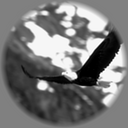
\includegraphics[scale = 0.26]{../../proposal/img3.png} & $\vec{x}_1 = $ 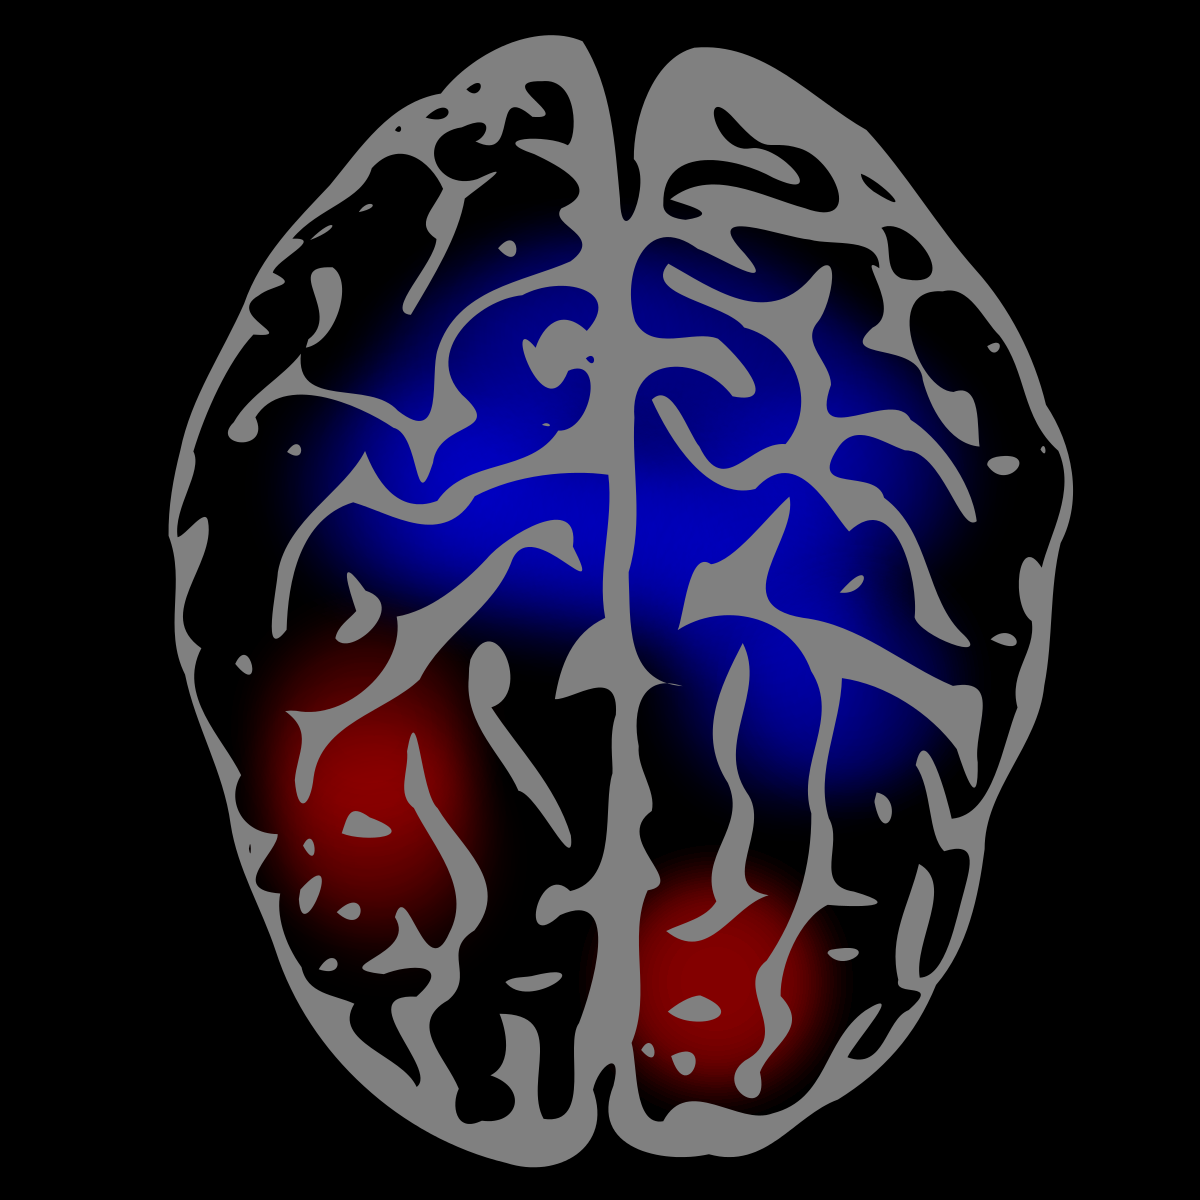
\includegraphics[scale = 0.035]{../../proposal/brain1.png} \\ \hline
2 & $y_2 = 2$ & 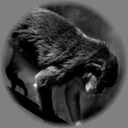
\includegraphics[scale = 0.26]{../../proposal/img4.png} & $\vec{x}_2 = $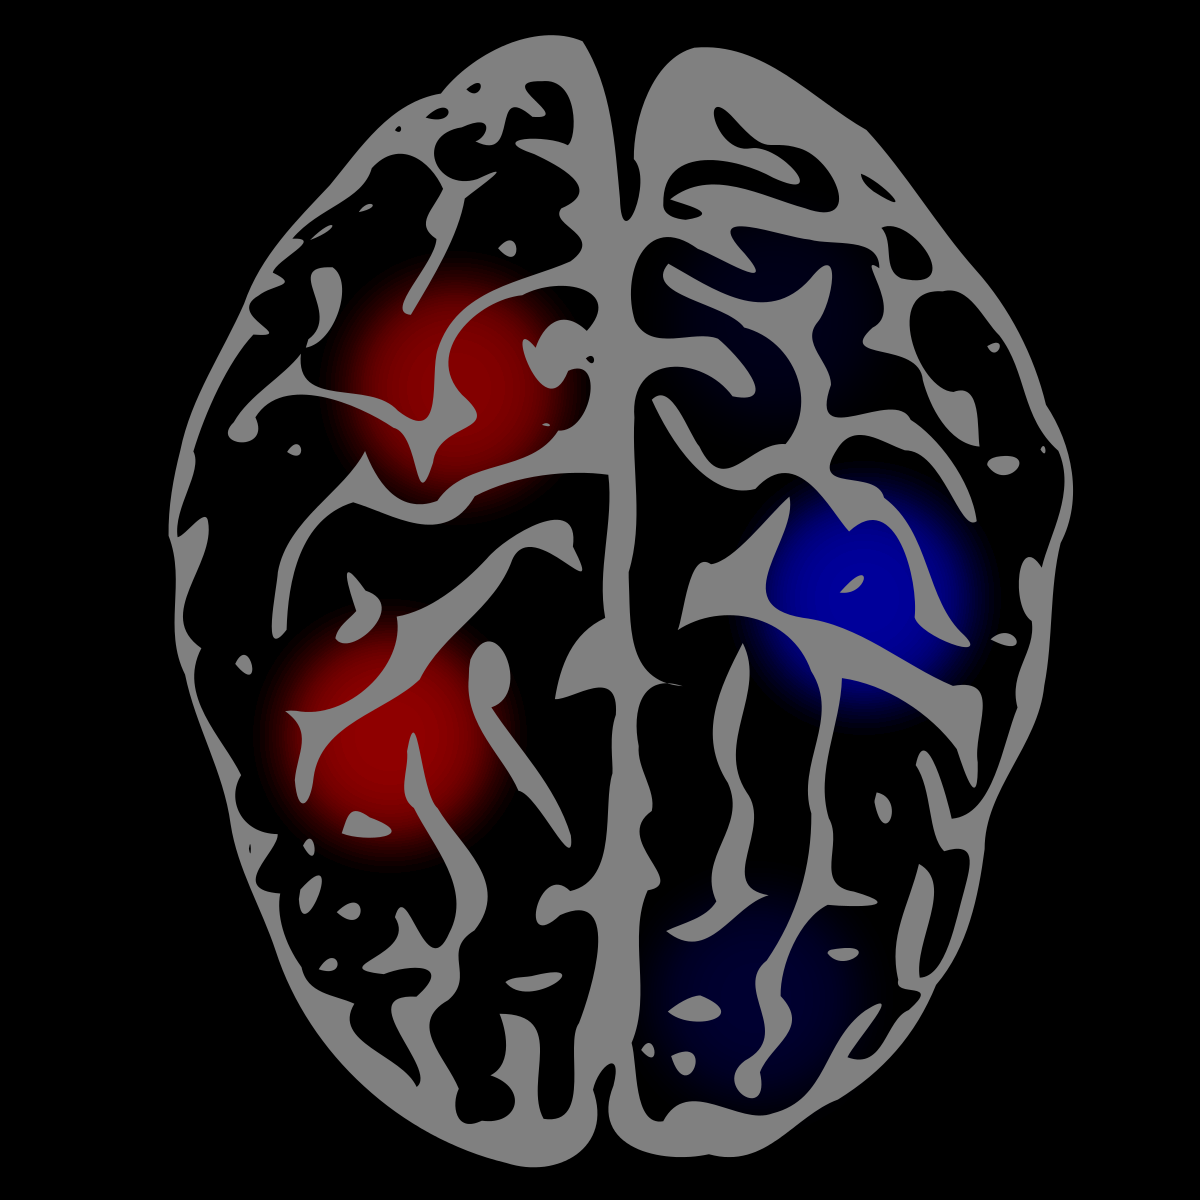
\includegraphics[scale = 0.035]{../../proposal/brain3.png} \\ \hline
3 & $y_3 = 1$ & 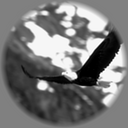
\includegraphics[scale = 0.26]{../../proposal/img3.png} & $\vec{x}_3 = $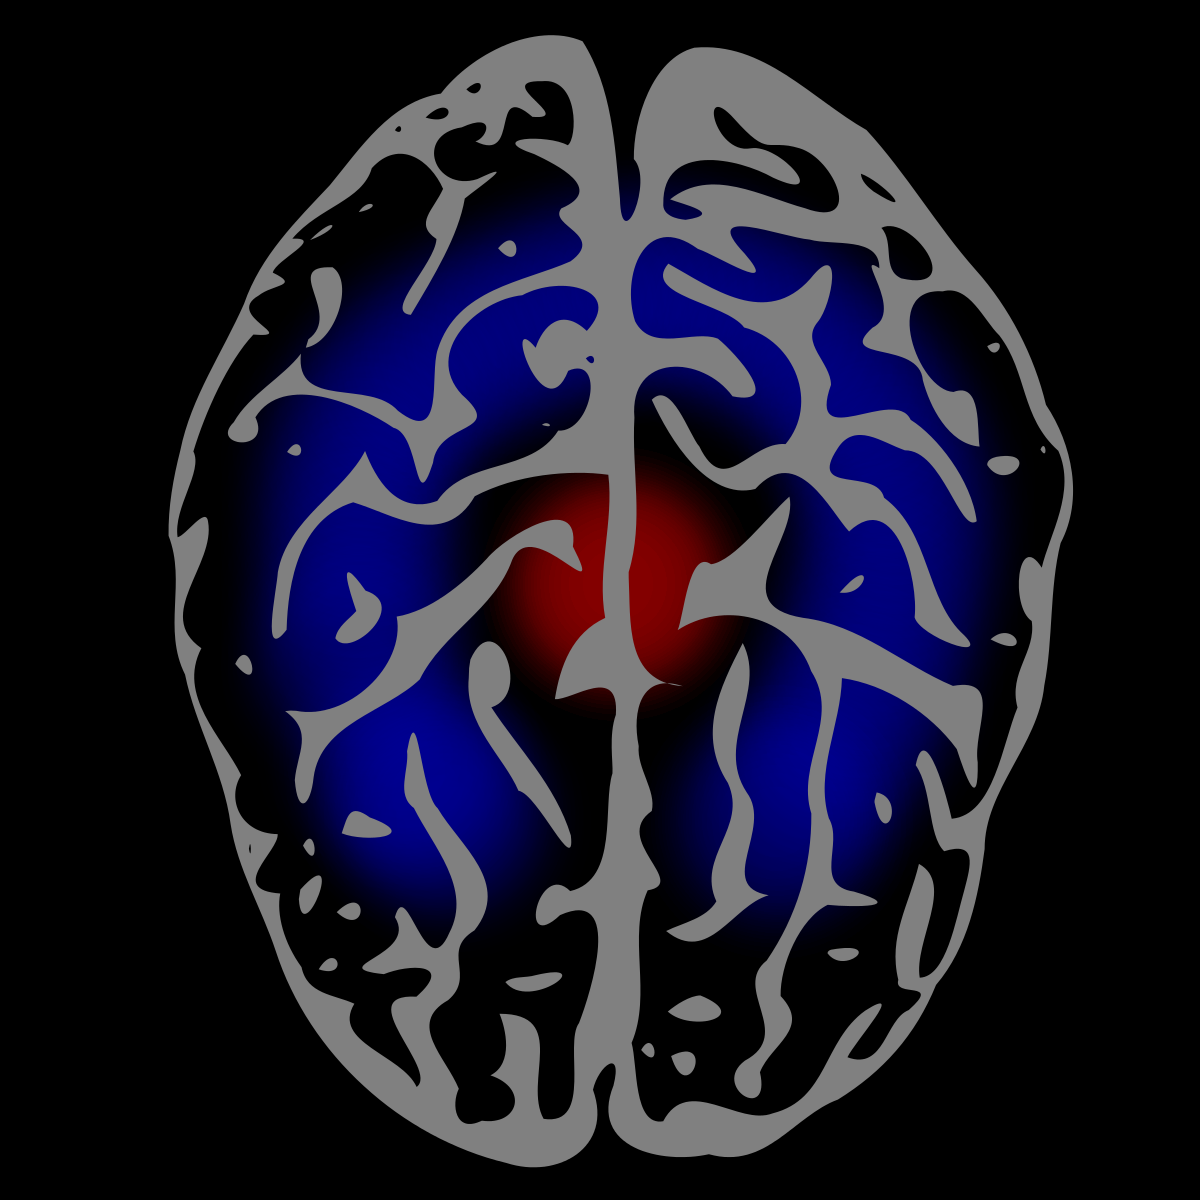
\includegraphics[scale = 0.035]{../../proposal/brain4.png} \\ \hline
4 & $y_4 = 2$ & 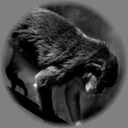
\includegraphics[scale = 0.26]{../../proposal/img4.png} & $\vec{x}_4 = $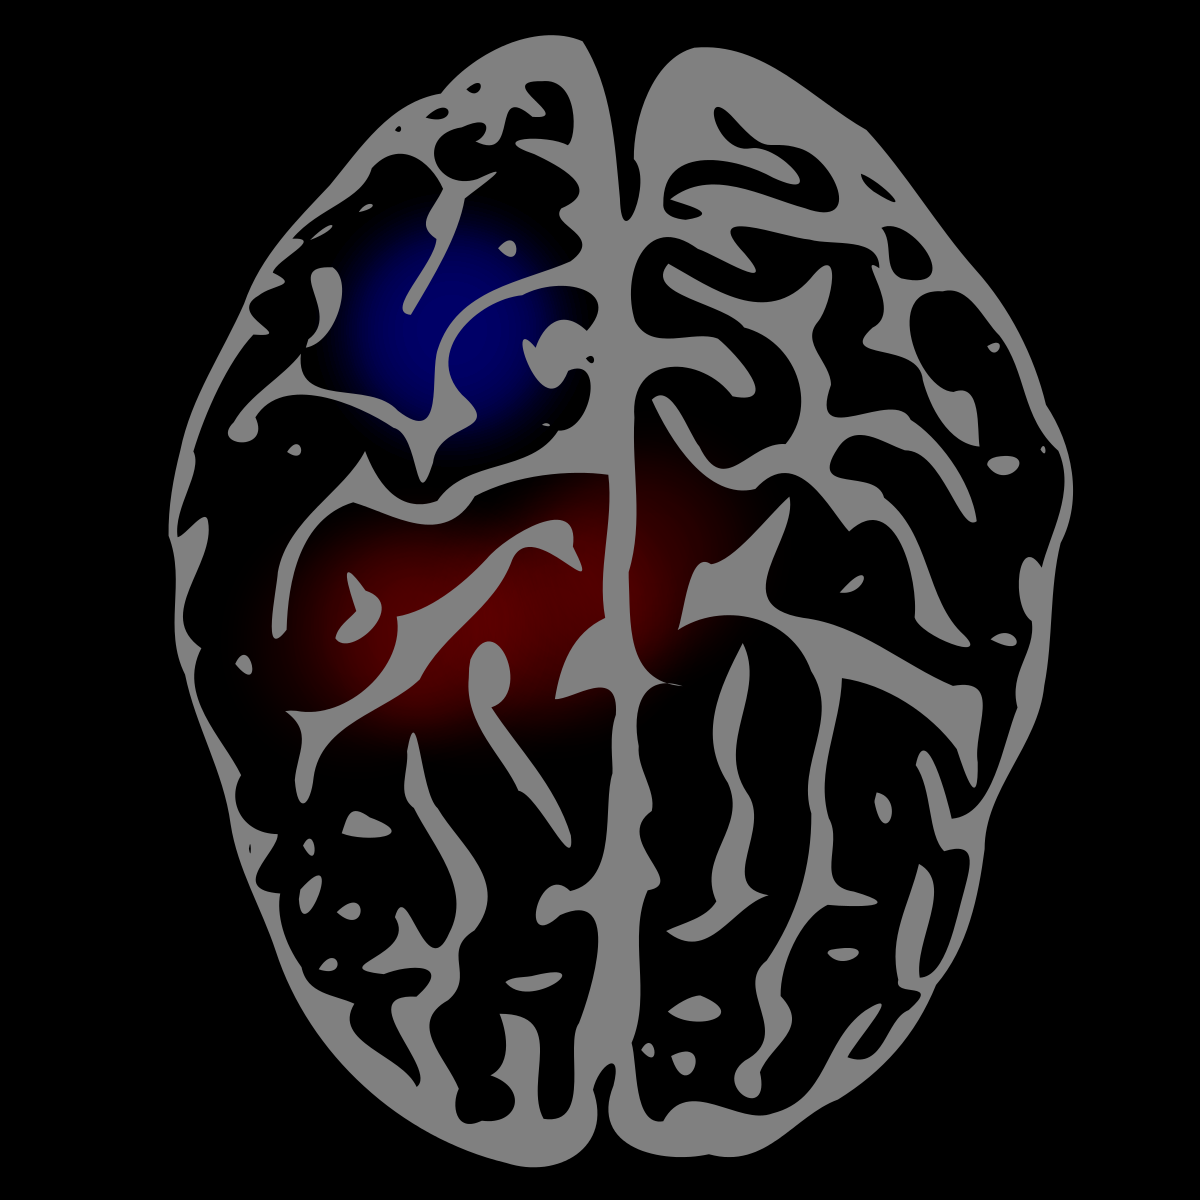
\includegraphics[scale = 0.035]{../../proposal/brain8.png} \\ \hline
\end{tabular}
\caption{Data output of a typical analysis of a task fMRI experiment.
  The raw data is processed to obtain a parametric map of inferred
  activation levels to each stimulus.  These activation levels are
  further utilized in downstream analyses. }
\label{fig:task_fmri}
\end{figure}

A number of statistical analyses can be performed on the
task-activation pairs $(y_i, \vec{x}_i)$.  The most common type of
analysis tests for significant \emph{peaks} of task-correlated
activity.  These analyses involve \emph{global} tests of the null
hypothesis of no correlation between task and activity.  However, MVPA
analyses tend to begin with local tests of independence between a
given region-of-interest (a cluster of neighboring voxels) and the
task.

\subsubsection{Classification-based test of independence}

A region of interest (ROI) is a collection of neighboring voxels,
chosen based on anatomical or geometric considerations.  To give a
concrete example, one can choose an arbitrary voxel in the brain, and
define an ROI as the set of all voxels within a given radius (say, $5
\text{mm}$) of the chosen voxel.  Recalling that $\vec{x}_i$ denotes
the activity level of the entire brain, let us write $\vec{x}_i^{ROI}$
for the subset of voxels in the brain map belonging to the ROI.

We would like to test the hypothesis of independence between the task
$Y$ and the joint activity level of the voxels belonging to the ROI,
considered as a random vector, $\vec{X}^{ROI}$.  While there are
numerous methods in the statistical literature for testing for
independence between a categorical random variable $Y$ and a random
vector $\vec{X}$, the approach taken in MVPA is typically to use
classification accuracies as the test statistic.

Recall that a classification rule is any (possibly stochastic) mapping
$f: \mathcal{X} \to \{1,\hdots, k\}$, where $k$ is the number of
levels of $Y$.  Let us assume that the $k$ different levels of $Y$
have the same number of repeats within the data.  The
\emph{generalization accuracy} of the classification rule is
\[
\text{GA}(f) = \frac{1}{k} \sum_{i=1}^k\Pr[f(\vec{X}^{ROI}) = i | Y = i].
\]
A trivial classification rule which outputs the result of a $k$-sided
die roll for all inputs $y$ would achieve a generalization accuracy of
$\text{GA} = \frac{1}{k}$.

Recall that the generalization accuracy of a data-dependent
classification rule $f$ can be obtained by using
\emph{data-splitting}, provided that the rule $f$ is constructed using
only the \emph{training data}.  Supposing that the original data
consists of pairs $(y_i,\vec{x}_i^{ROI})$ for $i = 1,\hdots, n$, let
$j_1,\hdots, j_{n_1}$ denote the $n_1$ randomly drawn training
indices, and $\ell_1,\hdots, \ell_{n_2}$ denote the $n_2$ randomly
drawn test indices.  The training data $(y_{j_i},
\vec{x}_{j_i}^{ROI})_{i=1}^{n_1}$ is used to construct a classification rule
$f$, while the test data is used to obtain a test accuracy $T$:
\[
T= \frac{1}{n_2} \sum_{i=1}^{n_2} I(f(\vec{x}_{\ell_i}^{ROI}) = y_{\ell_i}).
\]
%% also give the formula for stratifying by class

Under the null hypothesis $H_0: Y \perp \vec{X}^{ROI}$, the
generalization accuracy of any classification rule $f$ is equal to
$1/k$.  Therefore, we can write the null hypothesis as
\[
H_0: \text{GA}(f) = \frac{1}{k}
\]
and the alternative hypothesis as
\[
H_1: \text{GA}(f) > \frac{1}{k}.
\]

We will describe two different methods for testing $H_0$ versus $H_1$.
The first approach is to use the fact that the distribution of $T$ is
known under the null hypothesis.  The second approach is a permutation
test.  The permutation test is more computationally expensive, but has
important advantages in terms of family-wise error control, as we will
describe in the sequel. %% describe in the next subsubsection

\emph{First approach.} Under the null hypothesis, using the fact that
the test observations $(y_{\ell_i}, \vec{x}_{\ell_i})$ are identical
and independently distributed from the population distribution of
stimulus-activity pairs, we have
\[
T \sim_{H_0} \text{Bernoulli}(n_2, \frac{1}{k})
\]
Therefore, let $c_\alpha$ be the $(1-\alpha)$ quantile of a
$\text{Bernoulli}(n_2, \frac{1}{k})$ distribution.  To perform a
hypothesis test at level $\alpha$, reject the null $H_0$ if $T >
c_\alpha$ and accept otherwise.  Equivalently, define the $p$-value as
the area under the tail of the $\text{Bernoulli}(n_2,
\frac{1}{k})$ distribution to the right of $T$,
\[
p = \Pr[X > T| X \sim \text{Bernoulli}(n_2, \frac{1}{k})],
\]
and reject if and only if $p < \alpha$.

\emph{Second approach (permutation test).}  Permutation tests are
widely used in statistical applications: for a good introduction to
the subject, the reader is invited to consult
\cite{efron1994introduction}.  Under the null hypothesis of
independence between $Y$ and $\vec{X}^{ROI}$, the test statistic $T$
(the test accuracy on $n_2$ test observations) has a distribution that
is invariant under permutation of the labels $Y_1,\hdots, Y_n$.
Therefore, obtain $B$ samples of permutation test statistics
$T^{(1)},\hdots, T^{(B)}$ by the following procedure:
\begin{itemize}
\item[1.] For $i = 1,\hdots, B$, draw a random permutation $\sigma: n \to n$.
\item[2.] Use the pairs
  $(y_{\sigma_i},\vec{x}^{ROI}_{\sigma_i})_{i=1}^{n_1}$ to construct
  classification rule $f^{(i)}$ (using the same classifier as the one
  used to construct $f$).
\item[3.] Evaluate the test accuracy of $f^{(i)}$,
\[
T^{(i)}= \frac{1}{n_2} \sum_{i=1}^{n_2} I(f^{(i)}(\vec{x}_{\sigma_i}^{ROI}) = y_{\sigma_i}).
\]
\end{itemize}
The permutation $p$-value is calculated based on the rank of $T$ within the sample of permuation test statistics:
\[
p = \frac{\sum_{i=1}^B I(T^{(i)} < T) + 1}{B + 1},
\]
and reject the null hypothesis if and only if $p < \alpha$.

\subsubsection{Spotlight analysis}

\subsection{Other applications}

Experimentally, mutual information has been used to detect strong
dependencies between stimulus features and features derived from
neural recordings, which can be used to draw conclusions about the
kinds of stimuli that a neural subsystem is designed to detect, or to
distinguish between signal and noise in the neural output.
Theoretically, the assumption that neural systems maximize mutual
information between salient features of the stimulus and neural output
has allowed scientists to predict neural codes from signal processing
models: for instance, the center-surround structure of human retinal
neurons matches theoretical constructions for the optimal filter based
on correlations found in natural images [cite].


